% Options for packages loaded elsewhere
\PassOptionsToPackage{unicode}{hyperref}
\PassOptionsToPackage{hyphens}{url}
%
\documentclass[
]{article}
\usepackage{amsmath,amssymb}
\usepackage{iftex}
\ifPDFTeX
  \usepackage[T1]{fontenc}
  \usepackage[utf8]{inputenc}
  \usepackage{textcomp} % provide euro and other symbols
\else % if luatex or xetex
  \usepackage{unicode-math} % this also loads fontspec
  \defaultfontfeatures{Scale=MatchLowercase}
  \defaultfontfeatures[\rmfamily]{Ligatures=TeX,Scale=1}
\fi
\usepackage{lmodern}
\ifPDFTeX\else
  % xetex/luatex font selection
\fi
% Use upquote if available, for straight quotes in verbatim environments
\IfFileExists{upquote.sty}{\usepackage{upquote}}{}
\IfFileExists{microtype.sty}{% use microtype if available
  \usepackage[]{microtype}
  \UseMicrotypeSet[protrusion]{basicmath} % disable protrusion for tt fonts
}{}
\makeatletter
\@ifundefined{KOMAClassName}{% if non-KOMA class
  \IfFileExists{parskip.sty}{%
    \usepackage{parskip}
  }{% else
    \setlength{\parindent}{0pt}
    \setlength{\parskip}{6pt plus 2pt minus 1pt}}
}{% if KOMA class
  \KOMAoptions{parskip=half}}
\makeatother
\usepackage{xcolor}
\usepackage[margin=1in]{geometry}
\usepackage{longtable,booktabs,array}
\usepackage{calc} % for calculating minipage widths
% Correct order of tables after \paragraph or \subparagraph
\usepackage{etoolbox}
\makeatletter
\patchcmd\longtable{\par}{\if@noskipsec\mbox{}\fi\par}{}{}
\makeatother
% Allow footnotes in longtable head/foot
\IfFileExists{footnotehyper.sty}{\usepackage{footnotehyper}}{\usepackage{footnote}}
\makesavenoteenv{longtable}
\usepackage{graphicx}
\makeatletter
\def\maxwidth{\ifdim\Gin@nat@width>\linewidth\linewidth\else\Gin@nat@width\fi}
\def\maxheight{\ifdim\Gin@nat@height>\textheight\textheight\else\Gin@nat@height\fi}
\makeatother
% Scale images if necessary, so that they will not overflow the page
% margins by default, and it is still possible to overwrite the defaults
% using explicit options in \includegraphics[width, height, ...]{}
\setkeys{Gin}{width=\maxwidth,height=\maxheight,keepaspectratio}
% Set default figure placement to htbp
\makeatletter
\def\fps@figure{htbp}
\makeatother
\setlength{\emergencystretch}{3em} % prevent overfull lines
\providecommand{\tightlist}{%
  \setlength{\itemsep}{0pt}\setlength{\parskip}{0pt}}
\setcounter{secnumdepth}{-\maxdimen} % remove section numbering
\ifLuaTeX
  \usepackage{selnolig}  % disable illegal ligatures
\fi
\IfFileExists{bookmark.sty}{\usepackage{bookmark}}{\usepackage{hyperref}}
\IfFileExists{xurl.sty}{\usepackage{xurl}}{} % add URL line breaks if available
\urlstyle{same}
\hypersetup{
  pdftitle={SCGSR final report},
  hidelinks,
  pdfcreator={LaTeX via pandoc}}

\title{SCGSR final report}
\author{}
\date{\vspace{-2.5em}2023-06-21}

\begin{document}
\maketitle

\hypertarget{sample-summary}{%
\subsection{Sample Summary}\label{sample-summary}}

Soils from northwest Alaska were homogenized and pre-incubated at -2 and
-6 degrees Celsius for three months after which they were incubated at
2,4,6,8,10 degrees Celsius for one week. After the week long incubation
soils were extracted using 0.5M K2SO4, and chloroform extracted to
measure microbial biomass and nutrient concentrations. Sub-samples were
also sent to PNNL for MPLEx (Methanol chloroform extraction) to provide
more comprehensive analysis of the molecular composition of organic
matter using FT-ICR, NMR, GC-MS and LC-MS techniques. Lipidomics were
also performed to ascertain if there were any significant shifts in
microbial biomass.

\begin{center}\rule{0.5\linewidth}{0.5pt}\end{center}

\hypertarget{respiration-results}{%
\subsection{Respiration Results}\label{respiration-results}}

Respiration measurements were taken daily during the incubation using a
Li-850 bench top respiration unit. Below are the respiration rates for
each sample, as well as the calculates total C respired. Linear mixed
effects model showed significant respiration variation by incubation and
pre incubation temperatures. An asterisks indicates a significant
(p\textless= 0.05, ANOVA) difference in pre-incubation temperature.

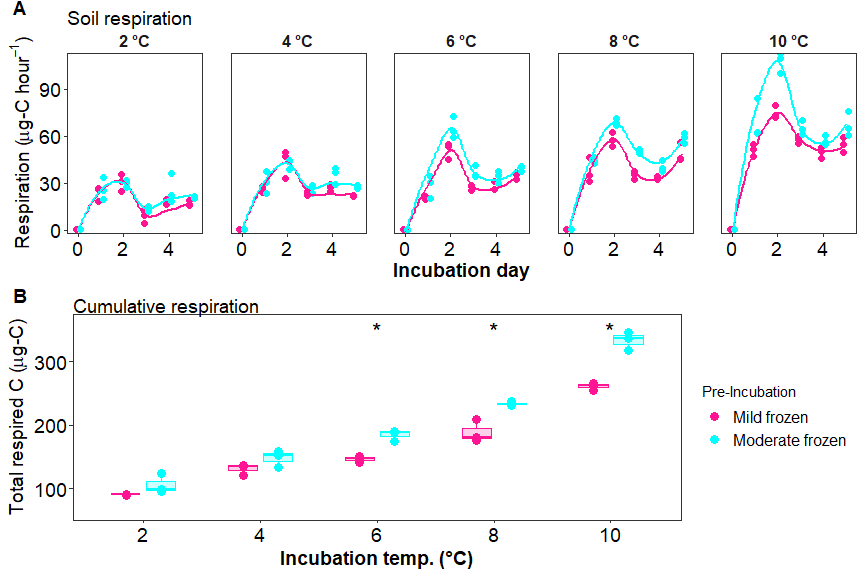
\includegraphics{SCGSR_Final_data_report_files/figure-latex/unnamed-chunk-1-1.pdf}

\begin{center}\rule{0.5\linewidth}{0.5pt}\end{center}

\hypertarget{soil-nutrients}{%
\subsection{Soil Nutrients}\label{soil-nutrients}}

Soil K2SO4 extracts were utilized to measure ammonium, Nitrate, Total
free primary amines, phosphate, Total reducing sugars. Below are the
concentration data. An asterisks indicates a significant (p\textless=
0.05, ANOVA) difference in pre-incubation temperature.

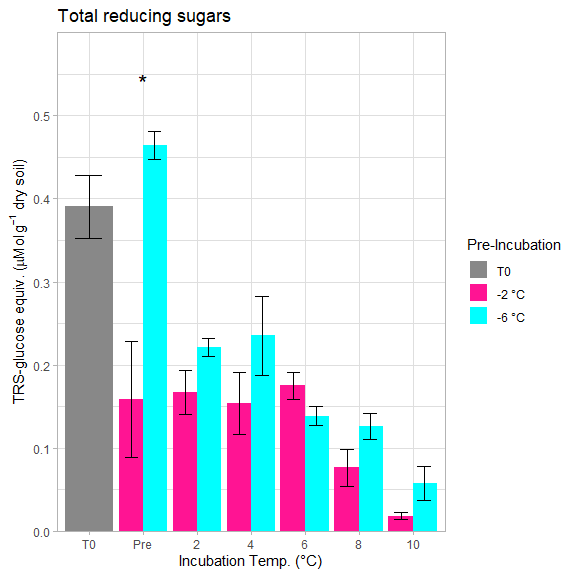
\includegraphics{SCGSR_Final_data_report_files/figure-latex/unnamed-chunk-2-1.pdf}
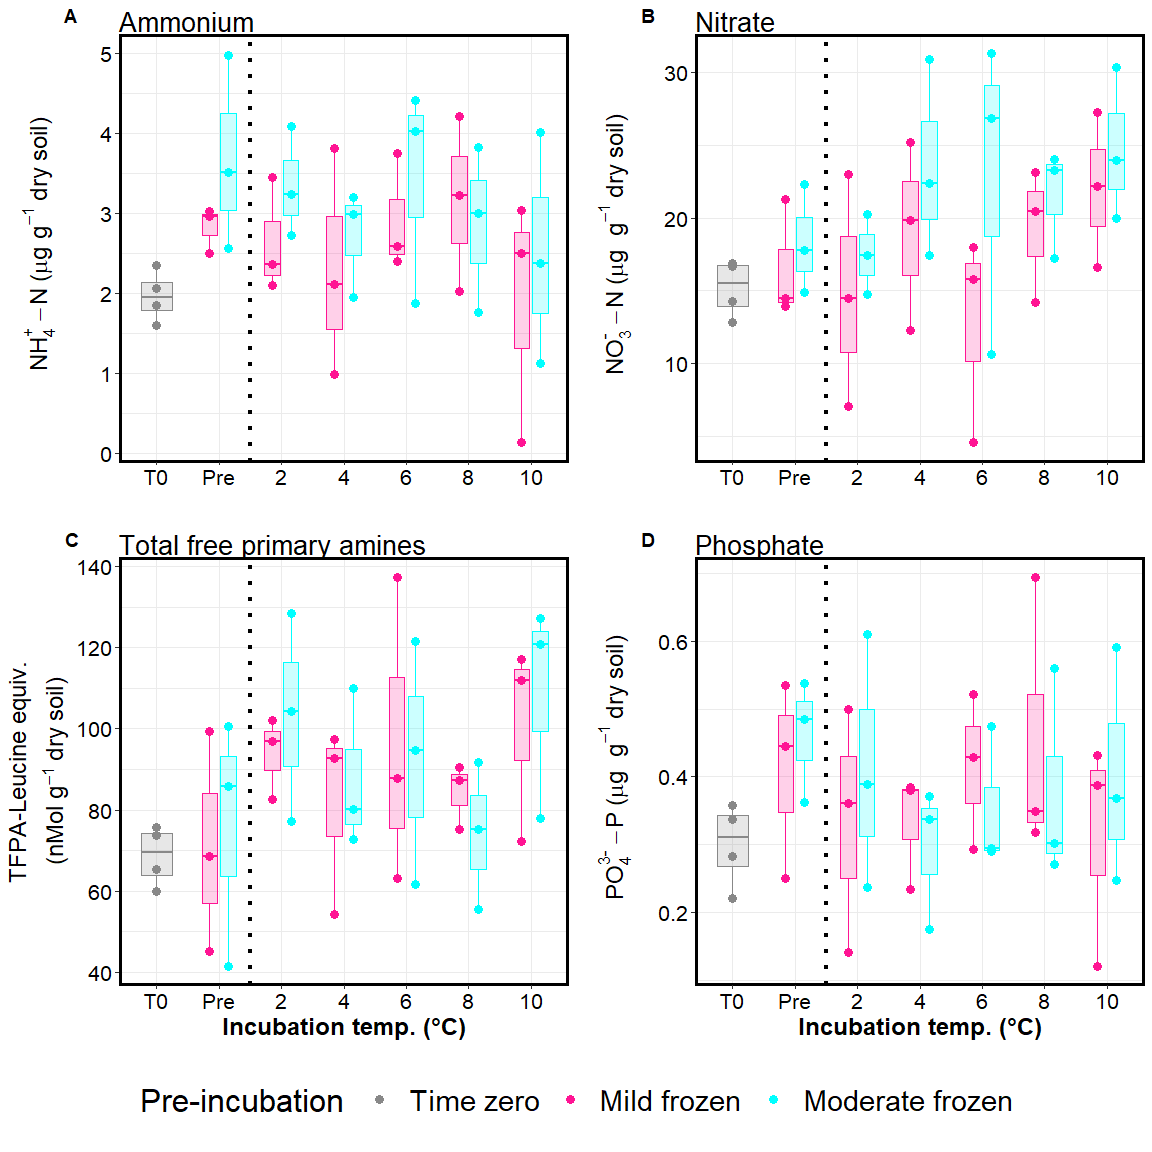
\includegraphics{SCGSR_Final_data_report_files/figure-latex/unnamed-chunk-3-1.pdf}

\begin{center}\rule{0.5\linewidth}{0.5pt}\end{center}

\hypertarget{microbial-biomass}{%
\subsection{Microbial Biomass}\label{microbial-biomass}}

Soil K2SO4 extracts were utilized to measure ammonium, Nitrate, Total
free primary amines, phosphate, Total reducing sugars. Below is the
concentration data.An asterisks indicates a significant (p\textless=
0.05,ANOVA) difference in pre-incubation temperature.

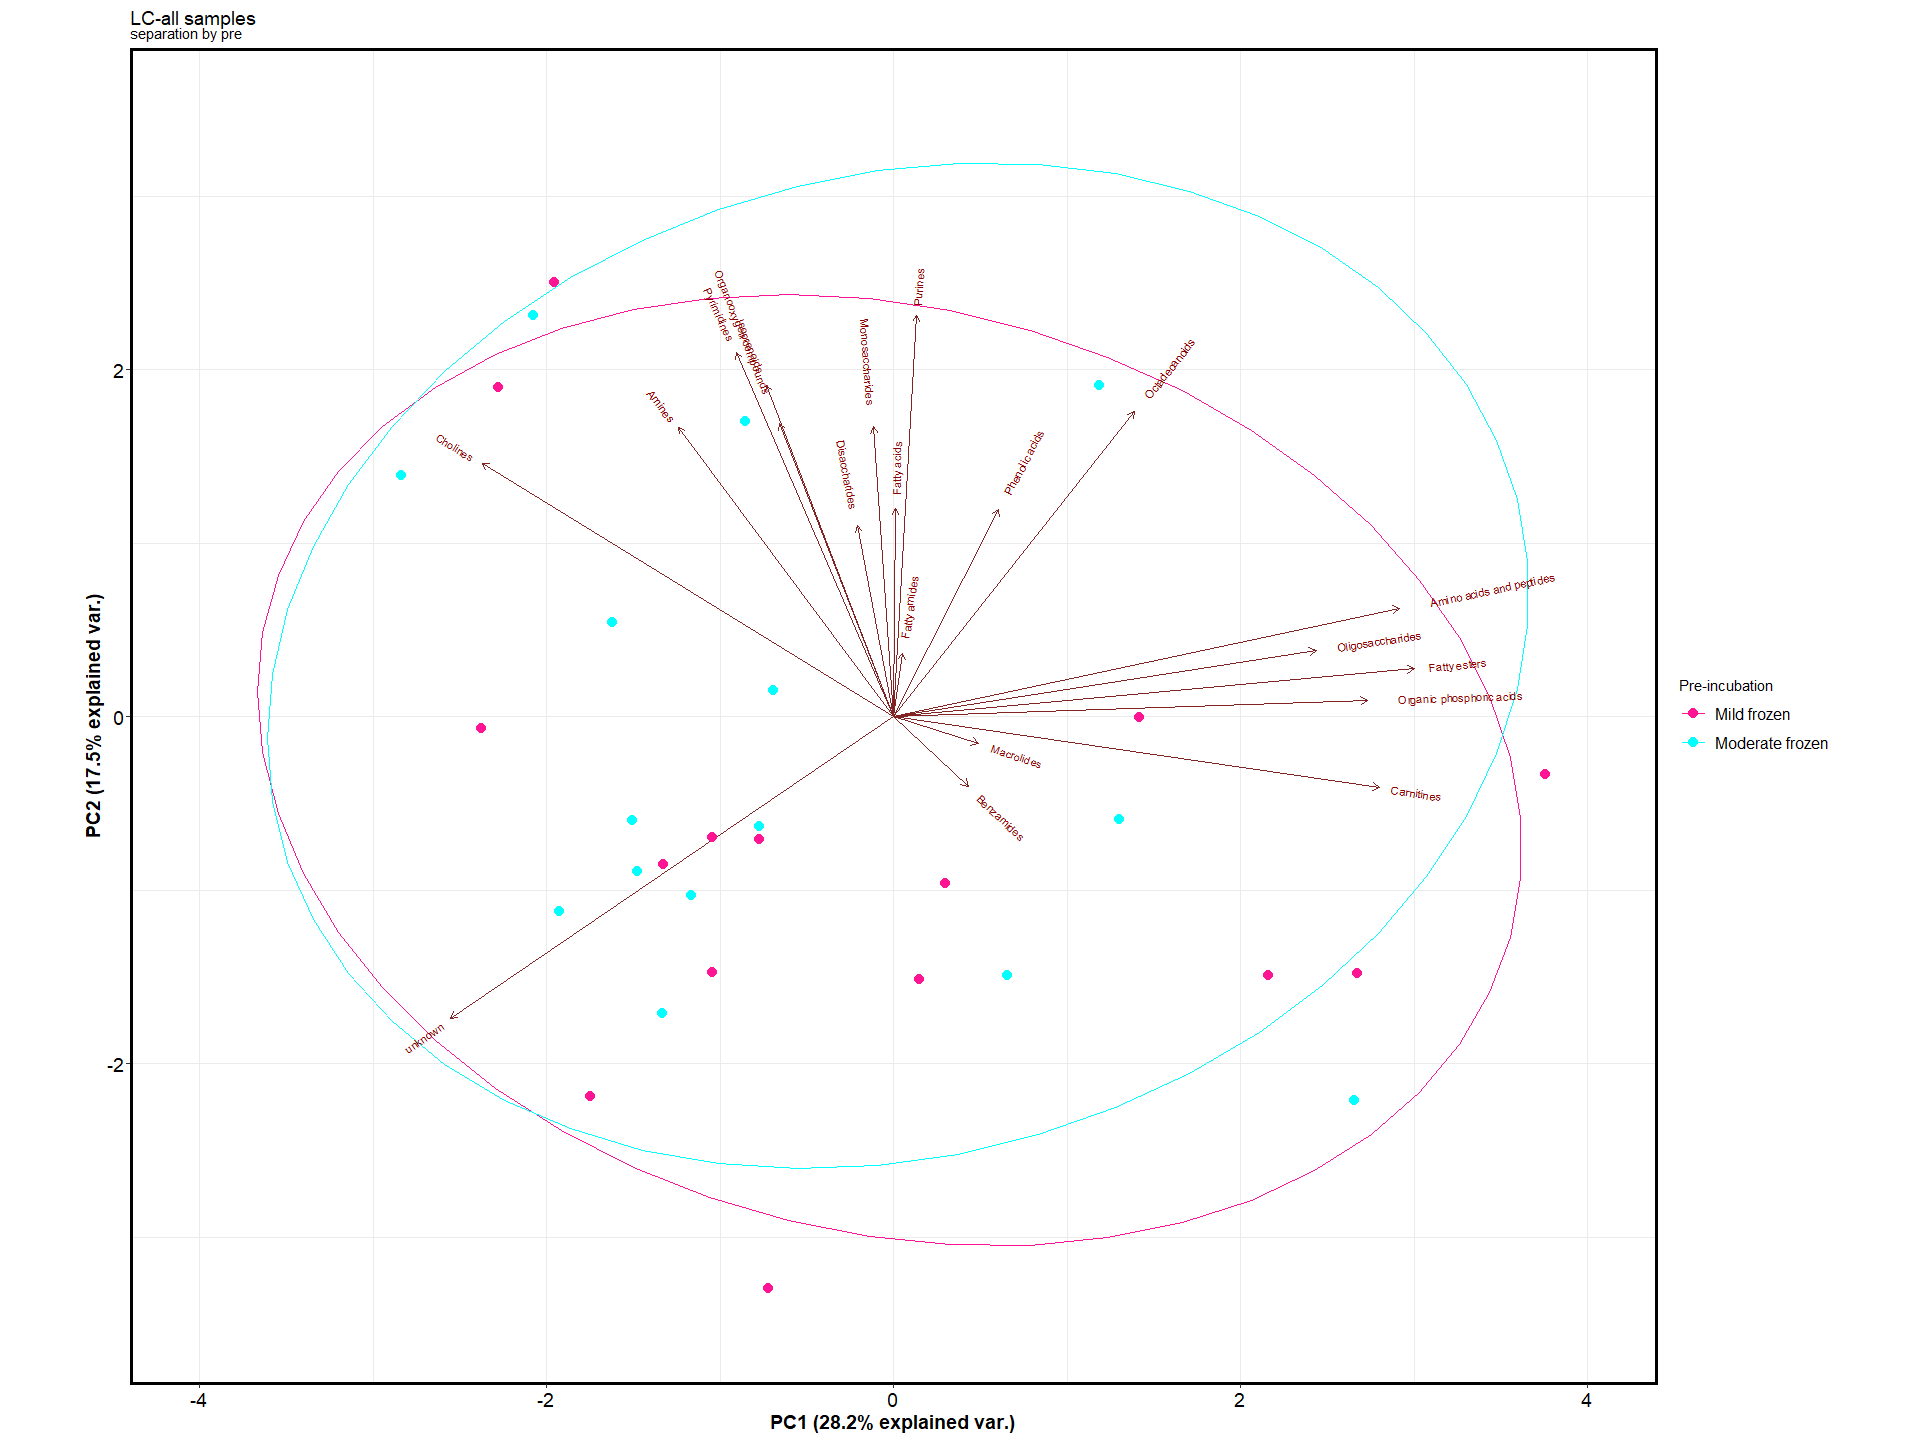
\includegraphics{SCGSR_Final_data_report_files/figure-latex/unnamed-chunk-4-1.pdf}

\begin{center}\rule{0.5\linewidth}{0.5pt}\end{center}

\hypertarget{gc-ms}{%
\subsection{GC-MS}\label{gc-ms}}

Below is the relative quantification of compounds identified by gas
chromatography within the MPLEx extracts.Little to no variation was
identified that corresponds to the more broad metrics above in the soil
nutrient section. The majority of compounds measured were unidentified.
Volcano plot can be used to identify the compounds that are
significantly greater between pre incubation temperature
(p\textless0.05, ANOVA). After which we used a PCA to visualize
separation between the pre incubation temperatures across significantly
different compounds. PERMANOVA results are displayed in the table below
the PCAs to show variation between treatments.

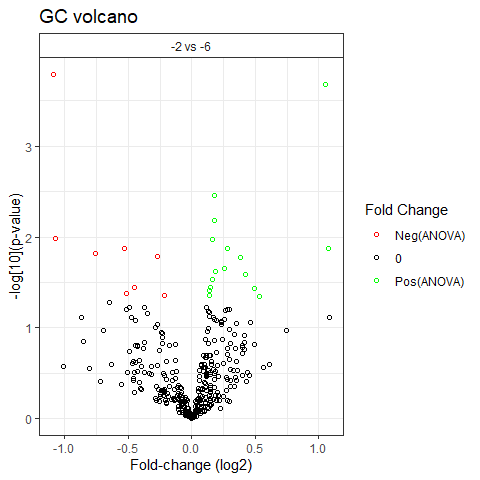
\includegraphics[width=1\linewidth]{SCGSR_Final_data_report_files/figure-latex/unnamed-chunk-5-1}

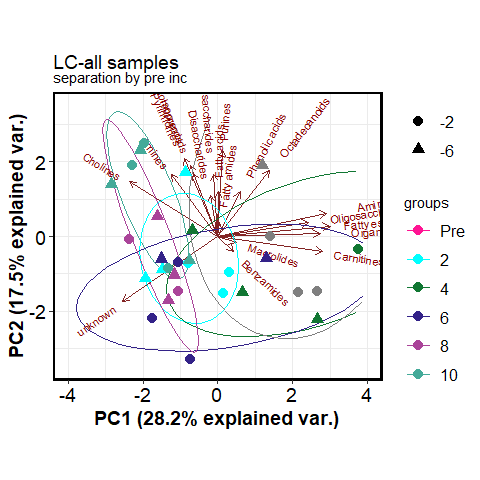
\includegraphics[width=0.5\linewidth]{SCGSR_Final_data_report_files/figure-latex/unnamed-chunk-6-1}
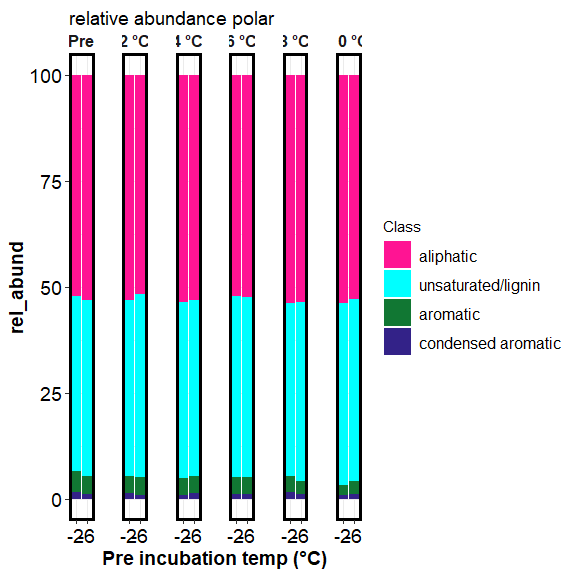
\includegraphics[width=0.5\linewidth]{SCGSR_Final_data_report_files/figure-latex/unnamed-chunk-6-2}

\begin{verbatim}
## NULL
\end{verbatim}

\begin{center}\rule{0.5\linewidth}{0.5pt}\end{center}

\hypertarget{lc-ms}{%
\subsection{LC-MS}\label{lc-ms}}

Below is the relative quantification of compounds identified by liquid
chromatography within the MPLEx extracts.Little to no variation was
identified that corresponds to the more broad metrics above in the soil
nutrient section. The majority of compounds measured were unidentified.
Volcano plot can be used to identify the compounds that are
significantly greater between pre incubation temperature
(p\textless0.05, ANOVA). After which we used a PCA to visualize
separation between the pre incubation temperatures across significantly
different compounds. PERMANOVA results are displayed in the table below
the PCAs to show variation between treatments.

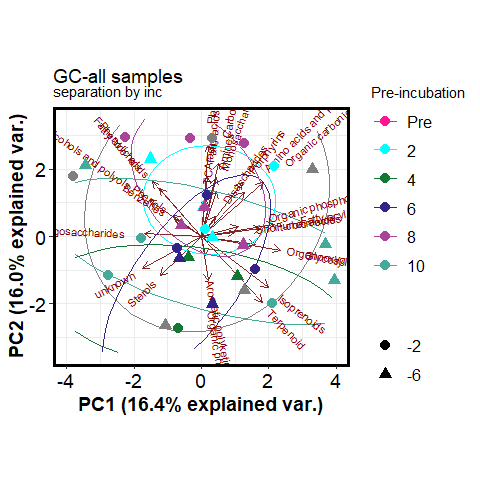
\includegraphics[width=1\linewidth]{SCGSR_Final_data_report_files/figure-latex/unnamed-chunk-8-1}

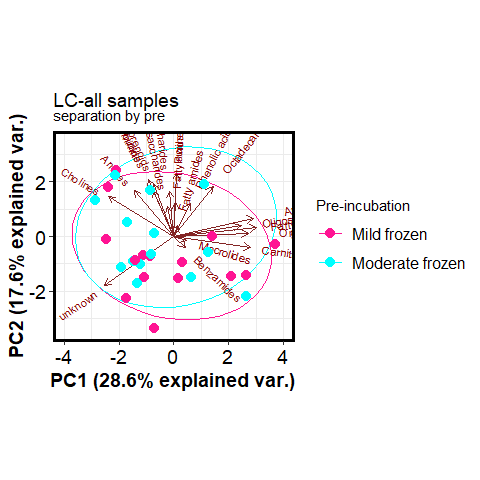
\includegraphics[width=0.5\linewidth]{SCGSR_Final_data_report_files/figure-latex/unnamed-chunk-9-1}
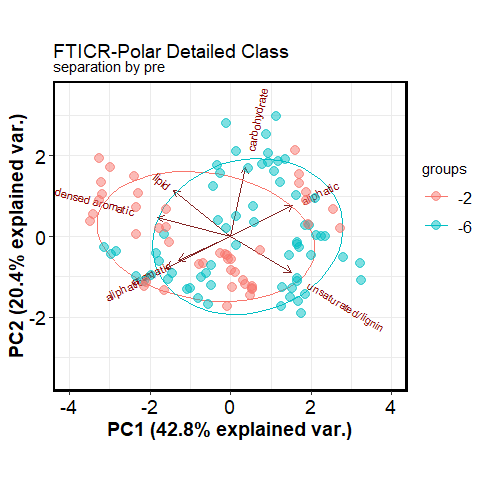
\includegraphics[width=0.5\linewidth]{SCGSR_Final_data_report_files/figure-latex/unnamed-chunk-9-2}

\begin{longtable}[]{@{}lrrrrr@{}}
\caption{Permanova results significant compounds only}\tabularnewline
\toprule\noalign{}
& Df & SumOfSqs & R2 & F & Pr(\textgreater F) \\
\midrule\noalign{}
\endfirsthead
\toprule\noalign{}
& Df & SumOfSqs & R2 & F & Pr(\textgreater F) \\
\midrule\noalign{}
\endhead
\bottomrule\noalign{}
\endlastfoot
pre & 1 & 0.0025136 & 0.1534787 & 7.235920 & 0.001 \\
inc & 5 & 0.0032903 & 0.2009044 & 1.894371 & 0.015 \\
pre:inc & 5 & 0.0025839 & 0.1577713 & 1.487660 & 0.098 \\
Residual & 23 & 0.0079896 & 0.4878455 & NA & NA \\
Total & 34 & 0.0163774 & 1.0000000 & NA & NA \\
\end{longtable}

\begin{center}\rule{0.5\linewidth}{0.5pt}\end{center}

\hypertarget{lipids}{%
\subsection{Lipids}\label{lipids}}

Lipid analysis was done via liquid chrometography on MEPLEx extracts.
Some variation was identified between pre-incubation temperatures,
though little was biologically significant. Conclusion that small
changes in biomass were present but not significant. A big missing piece
to this analysis would be community composition.Little no no variation
was observed within this data set. PCAs below show little to no
separation between incubation and pre incubation temperatures.

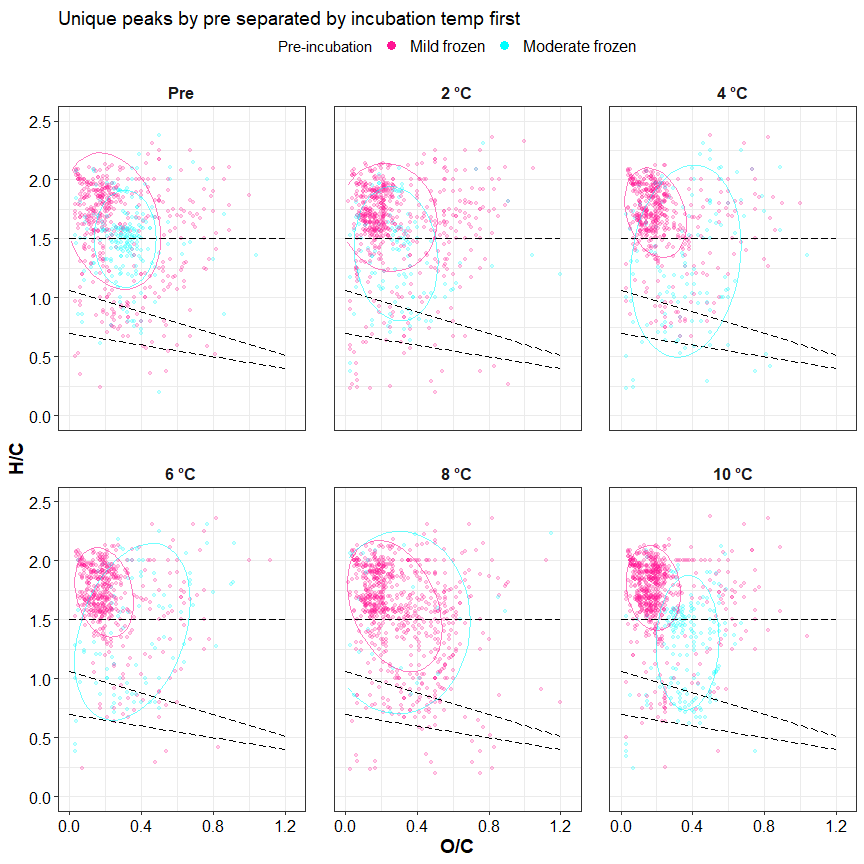
\includegraphics[width=0.5\linewidth]{SCGSR_Final_data_report_files/figure-latex/unnamed-chunk-11-1}
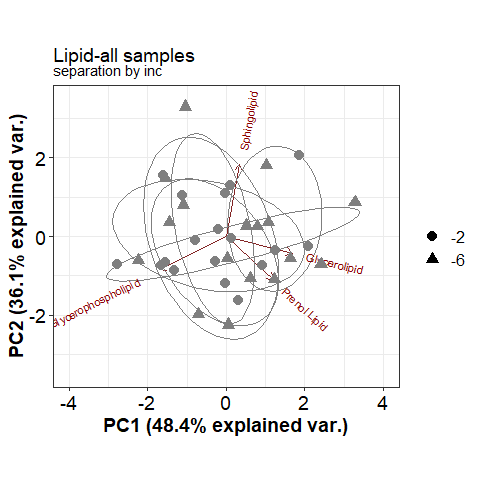
\includegraphics[width=0.5\linewidth]{SCGSR_Final_data_report_files/figure-latex/unnamed-chunk-11-2}

\begin{longtable}[]{@{}lrrrrr@{}}
\caption{Permanova results all}\tabularnewline
\toprule\noalign{}
& Df & SumOfSqs & R2 & F & Pr(\textgreater F) \\
\midrule\noalign{}
\endfirsthead
\toprule\noalign{}
& Df & SumOfSqs & R2 & F & Pr(\textgreater F) \\
\midrule\noalign{}
\endhead
\bottomrule\noalign{}
\endlastfoot
Pre & 1 & 0.0000127 & 0.0312988 & 1.259669 & 0.302 \\
Inc & 5 & 0.0000742 & 0.1823599 & 1.467871 & 0.175 \\
Pre:Inc & 5 & 0.0000773 & 0.1900165 & 1.529501 & 0.168 \\
Residual & 24 & 0.0002427 & 0.5963247 & NA & NA \\
Total & 35 & 0.0004071 & 1.0000000 & NA & NA \\
\end{longtable}

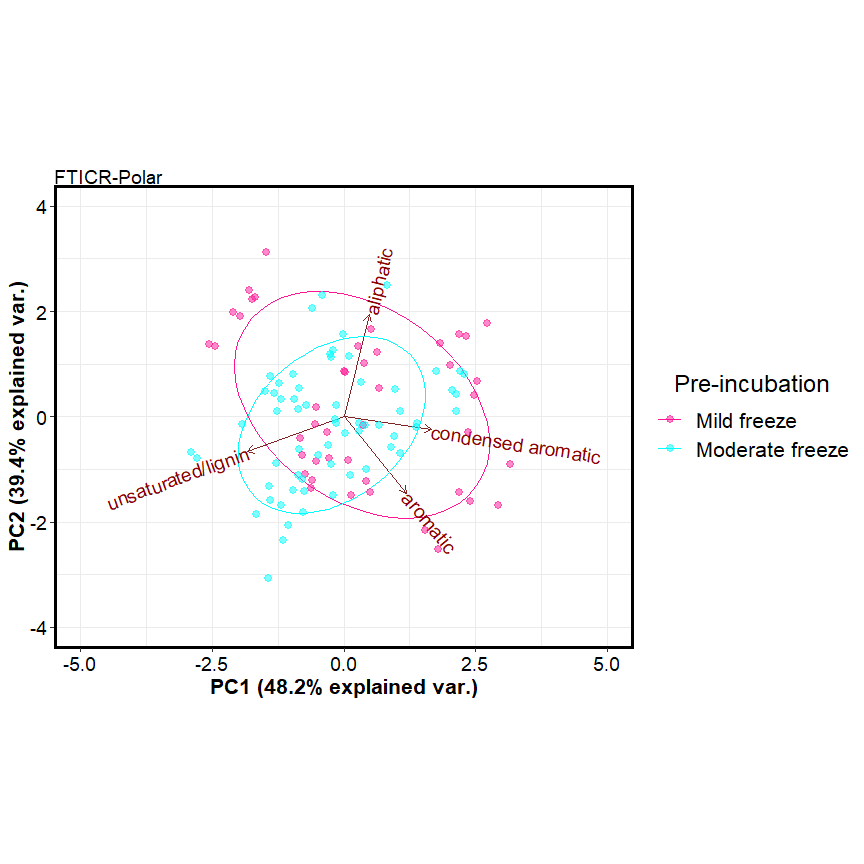
\includegraphics[width=0.5\linewidth]{SCGSR_Final_data_report_files/figure-latex/unnamed-chunk-13-1}
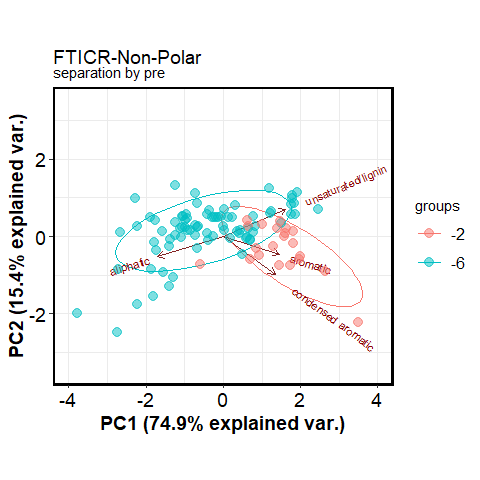
\includegraphics[width=0.5\linewidth]{SCGSR_Final_data_report_files/figure-latex/unnamed-chunk-13-2}

\begin{longtable}[]{@{}lrrrrr@{}}
\caption{Permanova results pos}\tabularnewline
\toprule\noalign{}
& Df & SumOfSqs & R2 & F & Pr(\textgreater F) \\
\midrule\noalign{}
\endfirsthead
\toprule\noalign{}
& Df & SumOfSqs & R2 & F & Pr(\textgreater F) \\
\midrule\noalign{}
\endhead
\bottomrule\noalign{}
\endlastfoot
Pre & 1 & 0.0000064 & 0.0153686 & 0.5551514 & 0.594 \\
Inc & 5 & 0.0000636 & 0.1537306 & 1.1106287 & 0.366 \\
Pre:Inc & 5 & 0.0000689 & 0.1664960 & 1.2028526 & 0.328 \\
Residual & 24 & 0.0002749 & 0.6644048 & NA & NA \\
Total & 35 & 0.0004138 & 1.0000000 & NA & NA \\
\end{longtable}

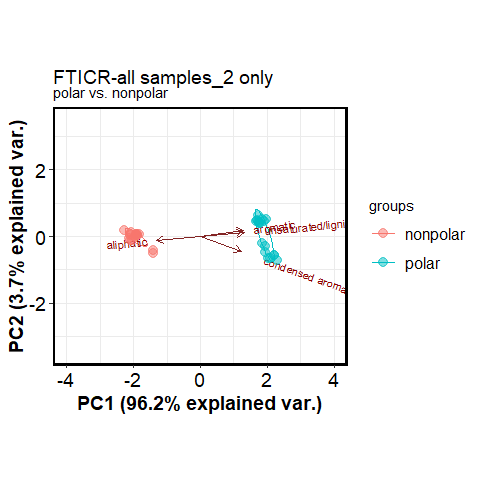
\includegraphics[width=0.5\linewidth]{SCGSR_Final_data_report_files/figure-latex/unnamed-chunk-15-1}
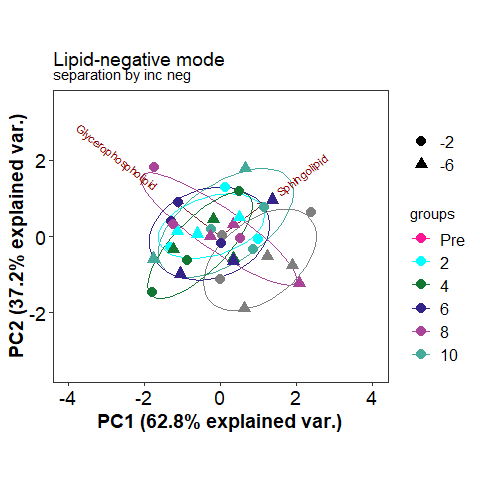
\includegraphics[width=0.5\linewidth]{SCGSR_Final_data_report_files/figure-latex/unnamed-chunk-15-2}

\begin{longtable}[]{@{}lrrrrr@{}}
\caption{Permanova results neg}\tabularnewline
\toprule\noalign{}
& Df & SumOfSqs & R2 & F & Pr(\textgreater F) \\
\midrule\noalign{}
\endfirsthead
\toprule\noalign{}
& Df & SumOfSqs & R2 & F & Pr(\textgreater F) \\
\midrule\noalign{}
\endhead
\bottomrule\noalign{}
\endlastfoot
Pre & 1 & 0.0000268 & 0.0346902 & 1.933659 & 0.170 \\
Inc & 5 & 0.0002308 & 0.2982330 & 3.324750 & 0.009 \\
Pre:Inc & 5 & 0.0001830 & 0.2365126 & 2.636681 & 0.035 \\
Residual & 24 & 0.0003332 & 0.4305642 & NA & NA \\
Total & 35 & 0.0007739 & 1.0000000 & NA & NA \\
\end{longtable}

\begin{center}\rule{0.5\linewidth}{0.5pt}\end{center}

\hypertarget{ft-ms-ft-icr}{%
\subsection{FT-MS (FT-ICR)}\label{ft-ms-ft-icr}}

FTICR was performed on MEPLEx extracts to gain a qualitative
understanding of the changes in organic matter composition after the
incubation. There appear to be differences between pre-incubation
temperatures, particularly in terms of the number of unique compounds,
which could be indicative of microbial processing of organic matter and
production of new organic compounds.

\hypertarget{fticr-van-krevelen-diagrams}{%
\subsubsection{FTICR Van krevelen
diagrams:}\label{fticr-van-krevelen-diagrams}}

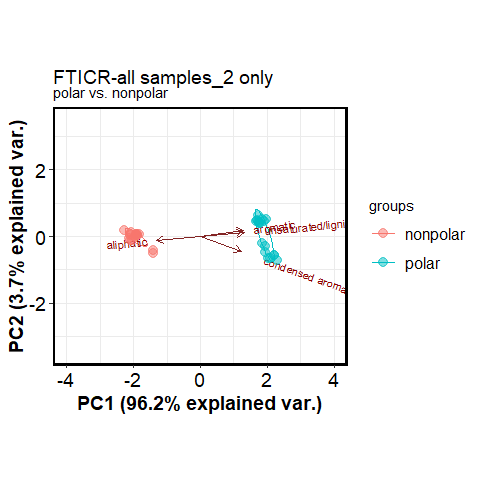
\includegraphics{SCGSR_Final_data_report_files/figure-latex/unnamed-chunk-17-1.pdf}

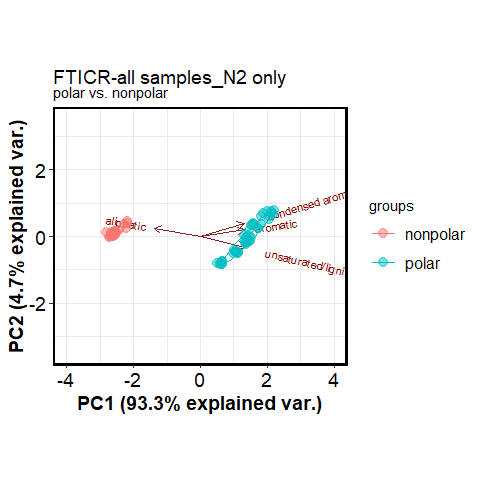
\includegraphics{SCGSR_Final_data_report_files/figure-latex/unnamed-chunk-18-1.pdf}

\hypertarget{fticr-common-vs-unique-peaks-by-treatment}{%
\subsubsection{FTICR Common vs unique peaks by
treatment:}\label{fticr-common-vs-unique-peaks-by-treatment}}

\hypertarget{all}{%
\paragraph{All}\label{all}}

\begin{verbatim}
## NULL
\end{verbatim}

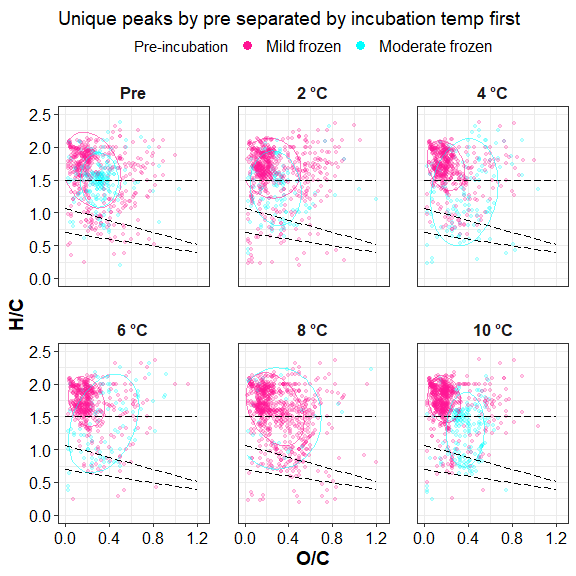
\includegraphics{SCGSR_Final_data_report_files/figure-latex/unnamed-chunk-19-1.pdf}

\begin{verbatim}
## NULL
\end{verbatim}

\begin{longtable}[]{@{}
  >{\raggedright\arraybackslash}p{(\columnwidth - 24\tabcolsep) * \real{0.2235}}
  >{\raggedleft\arraybackslash}p{(\columnwidth - 24\tabcolsep) * \real{0.0824}}
  >{\raggedleft\arraybackslash}p{(\columnwidth - 24\tabcolsep) * \real{0.0824}}
  >{\raggedleft\arraybackslash}p{(\columnwidth - 24\tabcolsep) * \real{0.0588}}
  >{\raggedleft\arraybackslash}p{(\columnwidth - 24\tabcolsep) * \real{0.0588}}
  >{\raggedleft\arraybackslash}p{(\columnwidth - 24\tabcolsep) * \real{0.0588}}
  >{\raggedleft\arraybackslash}p{(\columnwidth - 24\tabcolsep) * \real{0.0588}}
  >{\raggedleft\arraybackslash}p{(\columnwidth - 24\tabcolsep) * \real{0.0588}}
  >{\raggedleft\arraybackslash}p{(\columnwidth - 24\tabcolsep) * \real{0.0588}}
  >{\raggedleft\arraybackslash}p{(\columnwidth - 24\tabcolsep) * \real{0.0588}}
  >{\raggedleft\arraybackslash}p{(\columnwidth - 24\tabcolsep) * \real{0.0588}}
  >{\raggedleft\arraybackslash}p{(\columnwidth - 24\tabcolsep) * \real{0.0706}}
  >{\raggedleft\arraybackslash}p{(\columnwidth - 24\tabcolsep) * \real{0.0706}}@{}}
\caption{Unique between preincubation temperatures at each incubation
temperature}\tabularnewline
\toprule\noalign{}
\begin{minipage}[b]{\linewidth}\raggedright
Class
\end{minipage} & \begin{minipage}[b]{\linewidth}\raggedleft
-2\_Pre
\end{minipage} & \begin{minipage}[b]{\linewidth}\raggedleft
-6\_Pre
\end{minipage} & \begin{minipage}[b]{\linewidth}\raggedleft
-2\_2
\end{minipage} & \begin{minipage}[b]{\linewidth}\raggedleft
-6\_2
\end{minipage} & \begin{minipage}[b]{\linewidth}\raggedleft
-2\_4
\end{minipage} & \begin{minipage}[b]{\linewidth}\raggedleft
-6\_4
\end{minipage} & \begin{minipage}[b]{\linewidth}\raggedleft
-2\_6
\end{minipage} & \begin{minipage}[b]{\linewidth}\raggedleft
-6\_6
\end{minipage} & \begin{minipage}[b]{\linewidth}\raggedleft
-2\_8
\end{minipage} & \begin{minipage}[b]{\linewidth}\raggedleft
-6\_8
\end{minipage} & \begin{minipage}[b]{\linewidth}\raggedleft
-2\_10
\end{minipage} & \begin{minipage}[b]{\linewidth}\raggedleft
-6\_10
\end{minipage} \\
\midrule\noalign{}
\endfirsthead
\toprule\noalign{}
\begin{minipage}[b]{\linewidth}\raggedright
Class
\end{minipage} & \begin{minipage}[b]{\linewidth}\raggedleft
-2\_Pre
\end{minipage} & \begin{minipage}[b]{\linewidth}\raggedleft
-6\_Pre
\end{minipage} & \begin{minipage}[b]{\linewidth}\raggedleft
-2\_2
\end{minipage} & \begin{minipage}[b]{\linewidth}\raggedleft
-6\_2
\end{minipage} & \begin{minipage}[b]{\linewidth}\raggedleft
-2\_4
\end{minipage} & \begin{minipage}[b]{\linewidth}\raggedleft
-6\_4
\end{minipage} & \begin{minipage}[b]{\linewidth}\raggedleft
-2\_6
\end{minipage} & \begin{minipage}[b]{\linewidth}\raggedleft
-6\_6
\end{minipage} & \begin{minipage}[b]{\linewidth}\raggedleft
-2\_8
\end{minipage} & \begin{minipage}[b]{\linewidth}\raggedleft
-6\_8
\end{minipage} & \begin{minipage}[b]{\linewidth}\raggedleft
-2\_10
\end{minipage} & \begin{minipage}[b]{\linewidth}\raggedleft
-6\_10
\end{minipage} \\
\midrule\noalign{}
\endhead
\bottomrule\noalign{}
\endlastfoot
aliphatic & 313 & 114 & 465 & 49 & 402 & 56 & 408 & 46 & 520 & 14 & 566
& 60 \\
aromatic & 34 & 13 & 18 & 16 & 21 & 14 & 13 & 18 & 48 & 3 & 21 & 35 \\
condensed aromatic & 15 & 2 & 27 & 3 & NA & 18 & 9 & 3 & 25 & NA & 7 &
9 \\
unsaturated/lignin & 85 & 79 & 86 & 54 & 69 & 42 & 57 & 27 & 166 & 9 &
69 & 75 \\
\end{longtable}

\hypertarget{polar}{%
\paragraph{Polar}\label{polar}}

\begin{verbatim}
## NULL
\end{verbatim}

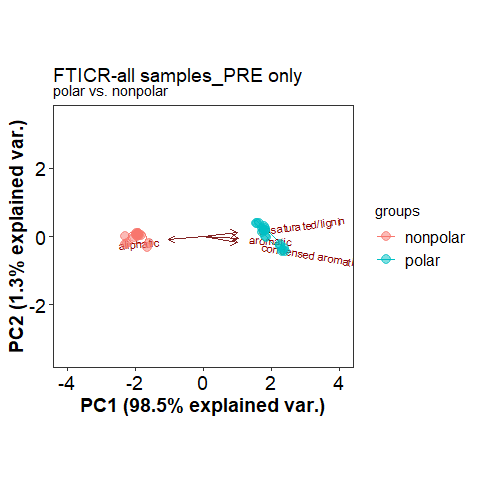
\includegraphics{SCGSR_Final_data_report_files/figure-latex/unnamed-chunk-20-1.pdf}

\begin{verbatim}
## NULL
\end{verbatim}

\begin{longtable}[]{@{}
  >{\raggedright\arraybackslash}p{(\columnwidth - 24\tabcolsep) * \real{0.2235}}
  >{\raggedleft\arraybackslash}p{(\columnwidth - 24\tabcolsep) * \real{0.0824}}
  >{\raggedleft\arraybackslash}p{(\columnwidth - 24\tabcolsep) * \real{0.0824}}
  >{\raggedleft\arraybackslash}p{(\columnwidth - 24\tabcolsep) * \real{0.0588}}
  >{\raggedleft\arraybackslash}p{(\columnwidth - 24\tabcolsep) * \real{0.0588}}
  >{\raggedleft\arraybackslash}p{(\columnwidth - 24\tabcolsep) * \real{0.0588}}
  >{\raggedleft\arraybackslash}p{(\columnwidth - 24\tabcolsep) * \real{0.0588}}
  >{\raggedleft\arraybackslash}p{(\columnwidth - 24\tabcolsep) * \real{0.0588}}
  >{\raggedleft\arraybackslash}p{(\columnwidth - 24\tabcolsep) * \real{0.0588}}
  >{\raggedleft\arraybackslash}p{(\columnwidth - 24\tabcolsep) * \real{0.0588}}
  >{\raggedleft\arraybackslash}p{(\columnwidth - 24\tabcolsep) * \real{0.0588}}
  >{\raggedleft\arraybackslash}p{(\columnwidth - 24\tabcolsep) * \real{0.0706}}
  >{\raggedleft\arraybackslash}p{(\columnwidth - 24\tabcolsep) * \real{0.0706}}@{}}
\caption{Unique between preincubation temperatures at each incubation
temperature polar}\tabularnewline
\toprule\noalign{}
\begin{minipage}[b]{\linewidth}\raggedright
Class
\end{minipage} & \begin{minipage}[b]{\linewidth}\raggedleft
-2\_Pre
\end{minipage} & \begin{minipage}[b]{\linewidth}\raggedleft
-6\_Pre
\end{minipage} & \begin{minipage}[b]{\linewidth}\raggedleft
-2\_2
\end{minipage} & \begin{minipage}[b]{\linewidth}\raggedleft
-6\_2
\end{minipage} & \begin{minipage}[b]{\linewidth}\raggedleft
-2\_4
\end{minipage} & \begin{minipage}[b]{\linewidth}\raggedleft
-6\_4
\end{minipage} & \begin{minipage}[b]{\linewidth}\raggedleft
-2\_6
\end{minipage} & \begin{minipage}[b]{\linewidth}\raggedleft
-6\_6
\end{minipage} & \begin{minipage}[b]{\linewidth}\raggedleft
-2\_8
\end{minipage} & \begin{minipage}[b]{\linewidth}\raggedleft
-6\_8
\end{minipage} & \begin{minipage}[b]{\linewidth}\raggedleft
-2\_10
\end{minipage} & \begin{minipage}[b]{\linewidth}\raggedleft
-6\_10
\end{minipage} \\
\midrule\noalign{}
\endfirsthead
\toprule\noalign{}
\begin{minipage}[b]{\linewidth}\raggedright
Class
\end{minipage} & \begin{minipage}[b]{\linewidth}\raggedleft
-2\_Pre
\end{minipage} & \begin{minipage}[b]{\linewidth}\raggedleft
-6\_Pre
\end{minipage} & \begin{minipage}[b]{\linewidth}\raggedleft
-2\_2
\end{minipage} & \begin{minipage}[b]{\linewidth}\raggedleft
-6\_2
\end{minipage} & \begin{minipage}[b]{\linewidth}\raggedleft
-2\_4
\end{minipage} & \begin{minipage}[b]{\linewidth}\raggedleft
-6\_4
\end{minipage} & \begin{minipage}[b]{\linewidth}\raggedleft
-2\_6
\end{minipage} & \begin{minipage}[b]{\linewidth}\raggedleft
-6\_6
\end{minipage} & \begin{minipage}[b]{\linewidth}\raggedleft
-2\_8
\end{minipage} & \begin{minipage}[b]{\linewidth}\raggedleft
-6\_8
\end{minipage} & \begin{minipage}[b]{\linewidth}\raggedleft
-2\_10
\end{minipage} & \begin{minipage}[b]{\linewidth}\raggedleft
-6\_10
\end{minipage} \\
\midrule\noalign{}
\endhead
\bottomrule\noalign{}
\endlastfoot
aliphatic & 100 & 126 & 122 & 50 & 67 & 74 & 57 & 63 & 265 & 13 & 46 &
105 \\
aromatic & 28 & 14 & 10 & 17 & 12 & 14 & 8 & 20 & 42 & 3 & 10 & 38 \\
condensed aromatic & 13 & 3 & 18 & 3 & NA & 18 & 7 & 3 & 24 & NA & 4 &
10 \\
unsaturated/lignin & 67 & 84 & 42 & 60 & 45 & 43 & 31 & 28 & 142 & 9 &
28 & 84 \\
\end{longtable}

\hypertarget{non-polar}{%
\paragraph{Non-Polar}\label{non-polar}}

\begin{verbatim}
## NULL
\end{verbatim}

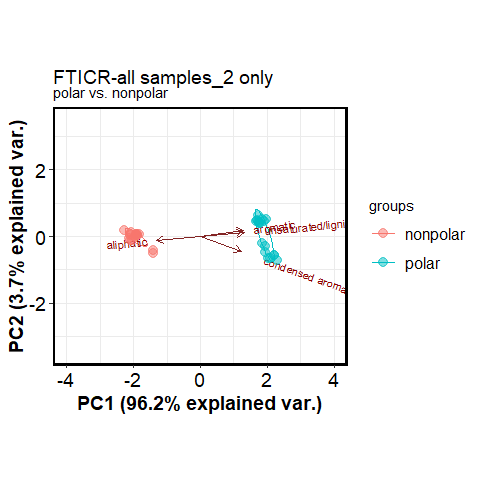
\includegraphics{SCGSR_Final_data_report_files/figure-latex/unnamed-chunk-21-1.pdf}

\begin{verbatim}
## NULL
\end{verbatim}

\begin{longtable}[]{@{}
  >{\raggedright\arraybackslash}p{(\columnwidth - 24\tabcolsep) * \real{0.2235}}
  >{\raggedleft\arraybackslash}p{(\columnwidth - 24\tabcolsep) * \real{0.0824}}
  >{\raggedleft\arraybackslash}p{(\columnwidth - 24\tabcolsep) * \real{0.0824}}
  >{\raggedleft\arraybackslash}p{(\columnwidth - 24\tabcolsep) * \real{0.0588}}
  >{\raggedleft\arraybackslash}p{(\columnwidth - 24\tabcolsep) * \real{0.0588}}
  >{\raggedleft\arraybackslash}p{(\columnwidth - 24\tabcolsep) * \real{0.0588}}
  >{\raggedleft\arraybackslash}p{(\columnwidth - 24\tabcolsep) * \real{0.0588}}
  >{\raggedleft\arraybackslash}p{(\columnwidth - 24\tabcolsep) * \real{0.0588}}
  >{\raggedleft\arraybackslash}p{(\columnwidth - 24\tabcolsep) * \real{0.0588}}
  >{\raggedleft\arraybackslash}p{(\columnwidth - 24\tabcolsep) * \real{0.0588}}
  >{\raggedleft\arraybackslash}p{(\columnwidth - 24\tabcolsep) * \real{0.0588}}
  >{\raggedleft\arraybackslash}p{(\columnwidth - 24\tabcolsep) * \real{0.0706}}
  >{\raggedleft\arraybackslash}p{(\columnwidth - 24\tabcolsep) * \real{0.0706}}@{}}
\caption{Unique between preincubation temperatures at each incubation
temperature nonpolar}\tabularnewline
\toprule\noalign{}
\begin{minipage}[b]{\linewidth}\raggedright
Class
\end{minipage} & \begin{minipage}[b]{\linewidth}\raggedleft
-2\_Pre
\end{minipage} & \begin{minipage}[b]{\linewidth}\raggedleft
-6\_Pre
\end{minipage} & \begin{minipage}[b]{\linewidth}\raggedleft
-2\_2
\end{minipage} & \begin{minipage}[b]{\linewidth}\raggedleft
-6\_2
\end{minipage} & \begin{minipage}[b]{\linewidth}\raggedleft
-2\_4
\end{minipage} & \begin{minipage}[b]{\linewidth}\raggedleft
-6\_4
\end{minipage} & \begin{minipage}[b]{\linewidth}\raggedleft
-2\_6
\end{minipage} & \begin{minipage}[b]{\linewidth}\raggedleft
-6\_6
\end{minipage} & \begin{minipage}[b]{\linewidth}\raggedleft
-2\_8
\end{minipage} & \begin{minipage}[b]{\linewidth}\raggedleft
-6\_8
\end{minipage} & \begin{minipage}[b]{\linewidth}\raggedleft
-2\_10
\end{minipage} & \begin{minipage}[b]{\linewidth}\raggedleft
-6\_10
\end{minipage} \\
\midrule\noalign{}
\endfirsthead
\toprule\noalign{}
\begin{minipage}[b]{\linewidth}\raggedright
Class
\end{minipage} & \begin{minipage}[b]{\linewidth}\raggedleft
-2\_Pre
\end{minipage} & \begin{minipage}[b]{\linewidth}\raggedleft
-6\_Pre
\end{minipage} & \begin{minipage}[b]{\linewidth}\raggedleft
-2\_2
\end{minipage} & \begin{minipage}[b]{\linewidth}\raggedleft
-6\_2
\end{minipage} & \begin{minipage}[b]{\linewidth}\raggedleft
-2\_4
\end{minipage} & \begin{minipage}[b]{\linewidth}\raggedleft
-6\_4
\end{minipage} & \begin{minipage}[b]{\linewidth}\raggedleft
-2\_6
\end{minipage} & \begin{minipage}[b]{\linewidth}\raggedleft
-6\_6
\end{minipage} & \begin{minipage}[b]{\linewidth}\raggedleft
-2\_8
\end{minipage} & \begin{minipage}[b]{\linewidth}\raggedleft
-6\_8
\end{minipage} & \begin{minipage}[b]{\linewidth}\raggedleft
-2\_10
\end{minipage} & \begin{minipage}[b]{\linewidth}\raggedleft
-6\_10
\end{minipage} \\
\midrule\noalign{}
\endhead
\bottomrule\noalign{}
\endlastfoot
aliphatic & 272 & 34 & 456 & 15 & 445 & 13 & 449 & 3 & 411 & 8 & 633 &
3 \\
aromatic & 13 & 1 & 13 & 1 & 14 & NA & 10 & NA & 11 & 1 & 20 & NA \\
condensed aromatic & 5 & NA & 11 & NA & 2 & NA & 3 & NA & 4 & NA & 4 &
NA \\
unsaturated/lignin & 49 & 20 & 111 & 3 & 77 & 6 & 102 & NA & 68 & 2 &
116 & 1 \\
\end{longtable}

\hypertarget{fticr-relative-abundance-and-pcas}{%
\subsubsection{FTICR relative abundance and
PCAs:}\label{fticr-relative-abundance-and-pcas}}

\hypertarget{relative-abundance}{%
\paragraph{Relative Abundance}\label{relative-abundance}}

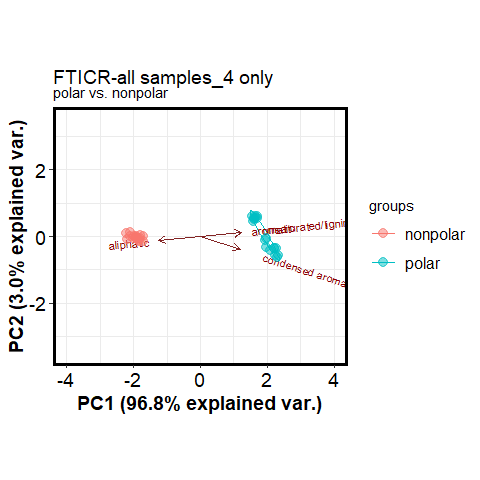
\includegraphics{SCGSR_Final_data_report_files/figure-latex/unnamed-chunk-22-1.pdf}
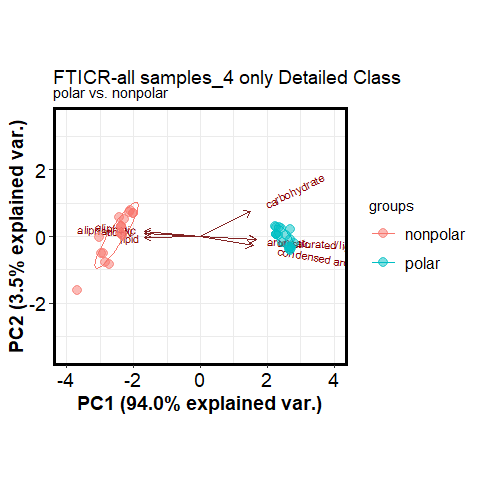
\includegraphics{SCGSR_Final_data_report_files/figure-latex/unnamed-chunk-22-2.pdf}
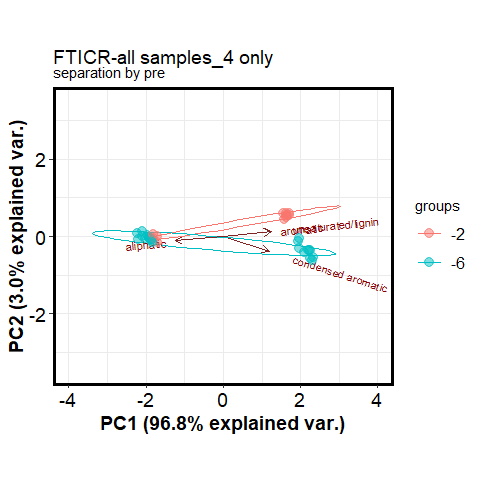
\includegraphics{SCGSR_Final_data_report_files/figure-latex/unnamed-chunk-22-3.pdf}

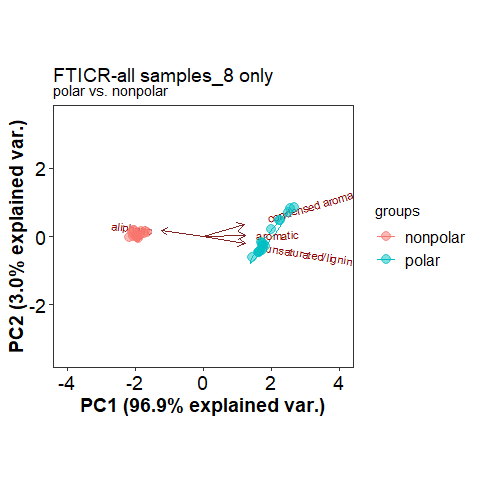
\includegraphics[width=0.5\linewidth]{SCGSR_Final_data_report_files/figure-latex/unnamed-chunk-24-1}
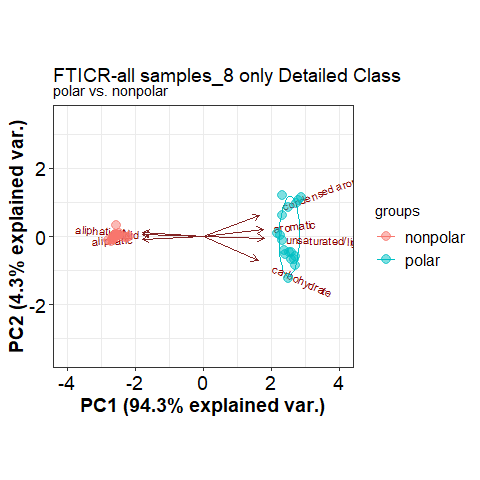
\includegraphics[width=0.5\linewidth]{SCGSR_Final_data_report_files/figure-latex/unnamed-chunk-24-2}

\begin{longtable}[]{@{}lrrrrr@{}}
\caption{Permanova results: Axis class Polar only}\tabularnewline
\toprule\noalign{}
& Df & SumOfSqs & R2 & F & Pr(\textgreater F) \\
\midrule\noalign{}
\endfirsthead
\toprule\noalign{}
& Df & SumOfSqs & R2 & F & Pr(\textgreater F) \\
\midrule\noalign{}
\endhead
\bottomrule\noalign{}
\endlastfoot
pre & 1 & 0.0004596 & 0.0321579 & 10.58298 & 0.001 \\
inc & 5 & 0.0066832 & 0.4676090 & 30.77754 & 0.001 \\
pre:inc & 5 & 0.0029803 & 0.2085238 & 13.72482 & 0.001 \\
Residual & 96 & 0.0041692 & 0.2917093 & NA & NA \\
Total & 107 & 0.0142922 & 1.0000000 & NA & NA \\
\end{longtable}

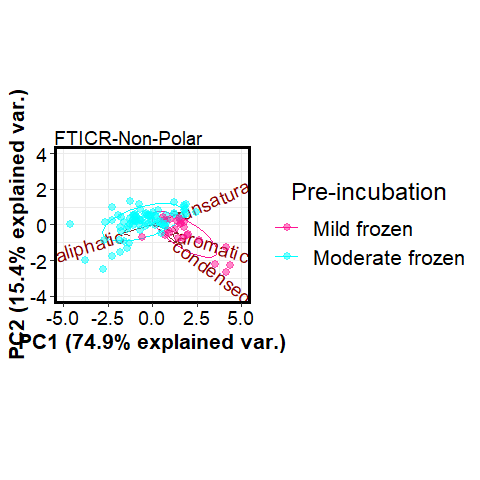
\includegraphics[width=0.5\linewidth]{SCGSR_Final_data_report_files/figure-latex/unnamed-chunk-26-1}
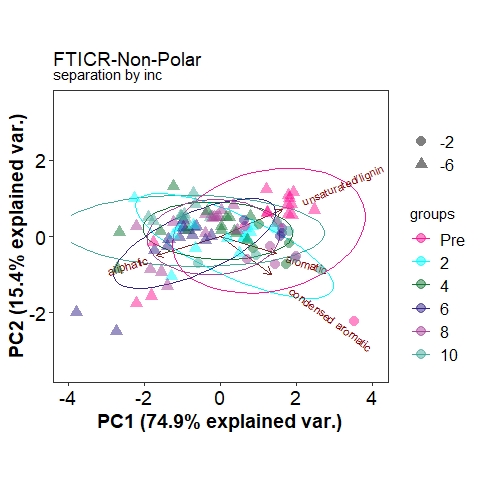
\includegraphics[width=0.5\linewidth]{SCGSR_Final_data_report_files/figure-latex/unnamed-chunk-26-2}

\begin{longtable}[]{@{}lrrrrr@{}}
\caption{Permanova results: Axis class Non-Polar only}\tabularnewline
\toprule\noalign{}
& Df & SumOfSqs & R2 & F & Pr(\textgreater F) \\
\midrule\noalign{}
\endfirsthead
\toprule\noalign{}
& Df & SumOfSqs & R2 & F & Pr(\textgreater F) \\
\midrule\noalign{}
\endhead
\bottomrule\noalign{}
\endlastfoot
pre & 1 & 0.0050061 & 0.1717359 & 26.4653827 & 0.001 \\
inc & 5 & 0.0052433 & 0.1798715 & 5.5438239 & 0.001 \\
pre:inc & 5 & 0.0009308 & 0.0319305 & 0.9841303 & 0.429 \\
Residual & 95 & 0.0179699 & 0.6164622 & NA & NA \\
Total & 106 & 0.0291500 & 1.0000000 & NA & NA \\
\end{longtable}

\begin{center}\rule{0.5\linewidth}{0.5pt}\end{center}

\hypertarget{session-info}{%
\subsection{Session Info}\label{session-info}}

Date run: 2023-08-25

\begin{verbatim}
## R version 4.2.3 (2023-03-15 ucrt)
## Platform: x86_64-w64-mingw32/x64 (64-bit)
## Running under: Windows 10 x64 (build 19045)
## 
## Matrix products: default
## 
## locale:
## [1] LC_COLLATE=English_United States.utf8 
## [2] LC_CTYPE=English_United States.utf8   
## [3] LC_MONETARY=English_United States.utf8
## [4] LC_NUMERIC=C                          
## [5] LC_TIME=English_United States.utf8    
## 
## attached base packages:
## [1] grid      stats     graphics  grDevices utils     datasets  methods  
## [8] base     
## 
## other attached packages:
##  [1] ropls_1.30.0        trelliscopejs_0.2.6 pmartR_2.4.0       
##  [4] agricolae_1.3-6     knitr_1.43          nlme_3.1-162       
##  [7] cowplot_1.1.1       ggpubr_0.6.0        janitor_2.2.0      
## [10] pracma_2.4.2        reshape2_1.4.4      ggbiplot_0.55      
## [13] scales_1.2.1        plyr_1.8.8          vegan_2.6-4        
## [16] lattice_0.20-45     permute_0.9-7       lubridate_1.9.2    
## [19] forcats_1.0.0       stringr_1.5.0       dplyr_1.1.2        
## [22] purrr_1.0.1         readr_2.1.4         tidyr_1.3.0        
## [25] tibble_3.2.1        ggplot2_3.4.1       tidyverse_2.0.0    
## [28] tarchetypes_0.7.7   targets_1.2.0      
## 
## loaded via a namespace (and not attached):
##   [1] backports_1.4.1             qqman_0.1.8                
##   [3] igraph_1.5.0                lazyeval_0.2.2             
##   [5] splines_4.2.3               AlgDesign_1.2.1            
##   [7] listenv_0.9.0               GenomeInfoDb_1.34.9        
##   [9] digest_0.6.33               foreach_1.5.2              
##  [11] htmltools_0.5.5             fansi_1.0.4                
##  [13] magrittr_2.0.3              checkmate_2.2.0            
##  [15] base64url_1.4               cluster_2.1.4              
##  [17] tzdb_0.4.0                  limma_3.54.2               
##  [19] globals_0.16.2              matrixStats_1.0.0          
##  [21] timechange_0.2.0            prettyunits_1.1.1          
##  [23] colorspace_2.1-0            haven_2.5.3                
##  [25] xfun_0.39                   callr_3.7.3                
##  [27] crayon_1.5.2                RCurl_1.98-1.12            
##  [29] jsonlite_1.8.7              iterators_1.0.14           
##  [31] glue_1.6.2                  gtable_0.3.3               
##  [33] zlibbioc_1.44.0             XVector_0.38.0             
##  [35] webshot_0.5.5               DelayedArray_0.24.0        
##  [37] questionr_0.7.8             car_3.1-2                  
##  [39] BiocGenerics_0.44.0         abind_1.4-5                
##  [41] rstatix_0.7.2               miniUI_0.1.1.1             
##  [43] Rcpp_1.0.11                 MultiDataSet_1.26.0        
##  [45] viridisLite_0.4.2           xtable_1.8-4               
##  [47] progress_1.2.2              mclust_6.0.0               
##  [49] stats4_4.2.3                httr_1.4.6                 
##  [51] htmlwidgets_1.6.2           calibrate_1.7.7            
##  [53] ellipsis_0.3.2              farver_2.1.1               
##  [55] pkgconfig_2.0.3             utf8_1.2.3                 
##  [57] labeling_0.4.2              tidyselect_1.2.0           
##  [59] rlang_1.1.1                 later_1.3.1                
##  [61] munsell_0.5.0               tools_4.2.3                
##  [63] cli_3.6.1                   generics_0.1.3             
##  [65] broom_1.0.5                 evaluate_0.21              
##  [67] fastmap_1.1.1               yaml_2.3.7                 
##  [69] processx_3.8.2              fs_1.6.2                   
##  [71] future.callr_0.8.1          future_1.33.0              
##  [73] mime_0.12                   ggExtra_0.10.0             
##  [75] compiler_4.2.3              rstudioapi_0.15.0          
##  [77] plotly_4.10.2               ggsignif_0.6.4             
##  [79] klaR_1.7-2                  stringi_1.7.12             
##  [81] highr_0.10                  ps_1.7.5                   
##  [83] Matrix_1.6-0                vctrs_0.6.3                
##  [85] pillar_1.9.0                lifecycle_1.0.3            
##  [87] furrr_0.3.1                 combinat_0.0-8             
##  [89] data.table_1.14.8           bitops_1.0-7               
##  [91] httpuv_1.6.11               GenomicRanges_1.50.2       
##  [93] R6_2.5.1                    promises_1.2.0.1           
##  [95] IRanges_2.32.0              parallelly_1.36.0          
##  [97] codetools_0.2-19            MASS_7.3-58.2              
##  [99] SummarizedExperiment_1.28.0 withr_2.5.0                
## [101] S4Vectors_0.36.2            autocogs_0.1.4             
## [103] GenomeInfoDbData_1.2.9      mgcv_1.8-42                
## [105] parallel_4.2.3              hms_1.1.3                  
## [107] MultiAssayExperiment_1.24.0 labelled_2.12.0            
## [109] rmarkdown_2.23              snakecase_0.11.0           
## [111] MatrixGenerics_1.10.0       carData_3.0-5              
## [113] DistributionUtils_0.6-0     Biobase_2.58.0             
## [115] shiny_1.7.4.1               base64enc_0.1-3
\end{verbatim}

\end{document}
